
\section{Objectives}
By the end of this lab work, students are expected to learn how to 

\begin{itemize}
\item test linear characteristics of a resistor (current vs. voltage graph)
\item determine resistance from current vs. voltage graph 
\item measure power in DC circuits and verify the maximum power transfer theorem. 
\end{itemize}

\section{Parts}
\label{sec:partsEx2}

\begin{enumerate}
\item Breadboard    
\item One $1~[\kilo\ohm]$ resistor
  
\item One $2.2~[\kilo\ohm]$ resistor 
\item One $5~[\kilo\ohm]$ potentiometer
% \item Digital multimeter (DMM).     %DC ammeter (0-10~\milli\ampere)  
\end{enumerate}                    %Give demonstration on DMM use as ammeter?



\section{Background}
\label{sec:background}
This experiment consists of two parts. In the first part, you are to use Ohm's law for  a simple DC circuit and determine the  resistance from the  current versus voltage graph for the circuit. In the second part, you are to determine the power dissipated by  a variable resistor and investigate the maximum power transfer theorem.

\subsection{Potentiometer}
Since you will be using a potentiometer (POT) for this experiment, it is important to know how a potentiometer (variable resistor) works. It is basically a three terminal device where the resistance between the outer terminals is fixed. The center terminal is a moving wiper that is connected to a rotary shaft.    The shaft is used to change the resistance between the center terminal and one of the outer terminals. Figure~\ref{fig:potAnnotated} shows the potentiometer as used in the laboratory along with its symbol.

%\todo[inline]{Include a figure of the potentiometer and its symbol.}

\begin{figure}[h]
    \centering
    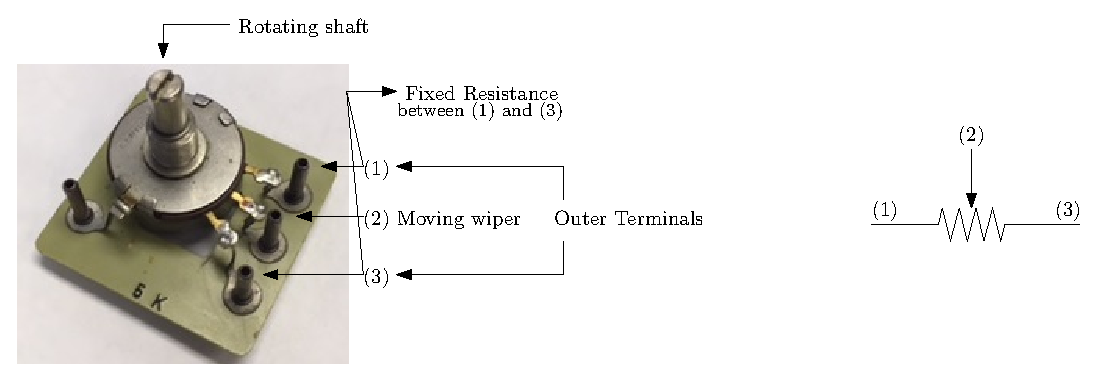
\includegraphics[scale=0.9]{figs/ipe/lab2/potAnnotated.eps}
    \caption{Potentiometer used in the experiment (left) and its symbol (right).}
    \label{fig:potAnnotated}
\end{figure}

The potentiometer is essentially a voltage divider where a portion of the applied voltage can be measured between the center and one of the outer terminals.



\subsection{Ohm's Law}
\label{sec:OhmsLaw}
For a fixed resistance in a branch of an electrical circuit, the current and voltage relationship follows Ohm's law, which states that -- \emph{at a constant temperature,  the current is proportional to the voltage across the resistor.}  Mathematically, it is described by %
%
\begin{align}
    I= \frac{V}{R},
\end{align}
where $I$ is the current flowing through the resistor, $V$ is the voltage across the terminals of the resistor, and $R$ is the resistance of the resistor. 

\begin{figure}[h]
    \centering
    \subfigure[][]{
      \label{fig:task1-Figure1-a}  
      \begin{circuitikz}
        \draw (0,0) to[V,l=$V_s$,invert,fill=green!50] (0,4*\smgrid)
        to[ammeter,v>=~,fill=yellow!50](10*\smgrid,4*\smgrid)
        to[R,v>=~,l=$R_1$,i=$I$](10*\smgrid,0) to[short,-*] (0,0)
        node[ground]{};
      \end{circuitikz}
    % \includegraphics[width=0.48\textwidth]{figs/ipe/lab2/task1-Figure1-a}
    }
    \subfigure[][]{
      \label{fig:task1-Figure1-b}
      \begin{circuitikz}[american]
        \draw (0,0) to[V,l^=$V_s$, invert,fill=green!50] (0,4*\smgrid)
        to[ammeter,v>=~,fill=yellow!50](10*\smgrid,4*\smgrid)
        to[R,v>=~,l=$R_2$,i=$I$](10*\smgrid,0) to[short,-*] (0,0)
        node[ground]{};
      \end{circuitikz}      
    % \includegraphics[width=0.48\textwidth]{figs/ipe/lab2/task1-Figure1-b}
    }
    \caption{Circuits for verifying Ohm's law using resistance~\subref{fig:task1-Figure1-a} $R_1$~and~\subref{fig:task1-Figure1-b} $R_2.$}
    \label{fig:task1-Figure1}
\end{figure}

In this part, you are to construct the circuits shown in Figure~\ref{fig:task1-Figure1} and use Ohm's law by applying different values of $V_s$ to the circuit using a variable power supply. 

% \begin{figure}[H]
%     \centering
    
%     \caption*{Figure 1(a): Circuit using Resistor $R_1$}
    
% \end{figure}

% \begin{figure}[H]
%     \centering
    
%     \caption*{Figure 1(b): Circuit using Resistor $R_2$}
    
% \end{figure}

\subsection{Maximum Power Transfer Theorem Verification}
\label{sec:maximumPowerTransferTheorem}

The current flowing through a resistor in a circuit converts the electrical energy into heat which is dissipated by the resistor. The rate at which the heat (energy) is dissipated from the resistor is the power, which is given by: %
$    P = VI = \frac{V^2}{R} = I^2R,$
%\end{align}
%
where $P$ is the power (unit: [\watt]~~or [\si{\joule\per\second}]), $V$ is the voltage across the resistor terminals, and $I$ is the current flowing through the resistance, $R.$ In this part, you will be constructing the circuit shown in Figure~\ref{fig:task2-Figure2} with $R_L$ being the load resistance. %
%
\begin{figure}[h]
  \centering
  \begin{circuitikz}[american]
    \draw
    % (0,0) to[V,l^=$V_s{=}12~{[}\volt{]}$,v<=](0,4*\smgrid) to[R,v>=$V_1$,l^=$R_1{=}1~{[}\kilo\ohm{]}$](10*\smgrid,4*\smgrid) to[variable american resistor,*-,v>=$V_2$,l=Use~$R_2{=}5~{[}\kilo\ohm{]}$ potentiometer](10*\smgrid,0) to[short,-*] (0,0)node[ground]{};
    (0,0) to[V,l^=$V_s$, invert,fill=green!50](0,4*\smgrid) to[R,v>=$V_1$,l^=$R_s$,i=$I$](10*\smgrid,4*\smgrid) to[variable american resistor,*-,v>=$V_L$,l^=$R_L$](10*\smgrid,0) to[short,-*] (0,0)node[ground]{};    
  \end{circuitikz}
    % \includegraphics[scale=1.5]{figs/ipe/lab2/task2-Figure2}
  \caption{DC circuit for verifying the maximum power transfer theorem.}
    \label{fig:task2-Figure2}
\end{figure}
%
You are to verify that the maximum power is delivered to the load resistor when the line resistance $R_s$ is equal to the load resistance $R_L.$  Note that, in practice, $R_s$ represents the internal source resistance associated with $V_s.$ However, it can also represent the resistance of a long transmission line. Using the circuit shown in Figure~\ref{fig:task2-Figure2}, the power delivered to the load resistor is computed as: %
%
%
\begin{subequations}
  \label{eq:PL}
  \begin{align}
    P_L &= V_LI = \frac{V_L^2}{R_L} = I^2R_L = \left[\frac{V_s}{R_s+R_L}\right]^2R_L,~~\text{with}\\
          I &=\frac{V_s}{R_T},
  \end{align}
\end{subequations}
%
where $V_L$ is the voltage across the load resistor $R_L$ and $R_T=R_s+R_L$ is
the equivalent resistance of the resistors ($R_s$ and $R_L$) connected in
series. 


\section{Prelab}
\label{sec:prelab}
Before starting to solve prelab problems, it is important to read the theoretical background illustrated in the previous section. The prelab is composed of two parts. In the first part, you are to use Ohm's law to predict the current for various source voltages. In the second part, the maximum power transfer theorem will be investigated for a given DC circuit using power computations. %
%
\begin{prelab}[Ohm's law]{prelab:OhmLaw}

  % Here you will predict the current of a circuit with two different values of a resistor.  
\begin{enumerate}
    \item Given the circuit shown in Figure~\ref{fig:task1-Figure1-a}, 
     \begin{enumerate}
         \item compute the currents for voltage $V_s=0,1,2,\ldots,15~[\volt]$ with $R_1=1~[\kilo\ohm],$
         \item use MATLAB to plot current $I$ (Y-axis) versus voltage $V_s$ (X-axis), and
           
         \item determine the resistance $R_1$ from the plot. 
         \end{enumerate}

    \item Given the circuit shown in Figure~\ref{fig:task1-Figure1-b}, 
     \begin{enumerate}
         \item compute the currents for voltage $V_s=0,1,2,\ldots,15~[\volt]$ with $R_2=2.2~[\kilo\ohm],$
         \item use MATLAB to plot current $I$ (Y-axis) versus voltage $V_s$ (X-axis), and
           
         \item determine the resistance $R_2$ from the plot. 
         \end{enumerate}
\end{enumerate}
 
\end{prelab}


\begin{prelab}[Maximum power transfer theorem]{prelab:maximumPowerTransferTheorem}
  %
Here, you will investigate the maximum power transfer theorem illustrated in section~\ref{sec:maximumPowerTransferTheorem}. Given the circuit shown in Figure~\ref{fig:task2-Figure2}:  %
 % 
     \begin{enumerate}
     \item Write the expression of the power, $P_L,$ delivered to the load resistor, $R_L,$ as a function of $V_s, R_s,$ and $R_L.$ %
       %
     \item What is the relation between $R_L$ and $R_s$ when the power delivered to the load resistor $R_L$ is maximum. Show your work in detail.
      % 
         \item Use MATLAB to plot the power $P_L$ (Y-axis) versus the load resistance $R_L$ (X-axis), for $V_s=12~[\volt],$ $R_s=1~[\kilo\ohm],$ and $R_L=0,0.1,0.2,\ldots,5~[\kilo\ohm].$
           
         \item Use the plot to determine the resistance $R_L$ when the power delivered to the load resistor is maximum. 
         \end{enumerate}
 
\end{prelab}

 
\section{Laboratory Work}

\subsection{Part~1}
\label{sec:part1}


\begin{enumerate}
\item Measure the values of the resistors and complete the following table.

  \begin{center}
  \begin{tabular}{c|c|c}
    \toprule
    Resistor &  Ideal (color-coded) & Measured\\
    \toprule                                        %      || Ideal || Measured || 
    $R_1$ & $\ldots$ & $\ldots$\\                   %  R1  || 1.0kΩ || 0.985kΩ  ||
    $R_2$ & $\ldots$ & $\ldots$\\                   %  R2  || 2.2kΩ || 2.193kΩ  ||
    POT (outer terminals) & $5~[\kilo\ohm]$ & $\ldots$\\   %  POT || 5kΩ   ||          ||   
    \bottomrule
  \end{tabular}    
  \end{center}


  
\item Construct the circuit shown in Figure~\ref{fig:task1-Figure1-a} with $R_1=1~[\kilo\ohm]$ and complete the following table:
  \begin{center}
  \begin{tabular}{|l|l|l|l|l|l|l|}
    \toprule
    $V_s=$ &  $2.0~[\volt]$ & $4.0~[\volt]$ & $6.0~[\volt]$ & $8.0~[\volt]$ &$10.0~[\volt]$ & $12.0~[\volt]$ \\                            % Figure 1(a)
    \hline                     % Vs   = ||2.0V ||4.0V ||6.0V ||8.0V ||10.0V ||12.0V ||
    $I = $   & & & & & &\\     % Im   = ||2.0mA||4.3mA||6.1mA||8.1mA||10.1mA||12.2mA|| Measured
    \bottomrule                % Ii   = ||2.0mA||4.0mA||6.0mA||8.0mA||10.0mA||12.0mA|| Ideal
  \end{tabular}      
  \end{center}

  \begin{mdframed}[roundcorner=5pt,backgroundcolor=yellow!50]
    Before you apply power, check with the Professor or the TA to verify your circuit is correct. 
  \end{mdframed}
  
\item Construct the circuit shown in Figure~\ref{fig:task1-Figure1-b} with $R_1=2.2~[\kilo\ohm]$ and complete the following table: %
%
  \begin{center}
  \begin{tabular}{|l|l|l|l|l|l|l|}
    \toprule
    $V_s=$ &  $2.0~[\volt]$ & $4.0~[\volt]$ & $6.0~[\volt]$ & $8.0~[\volt]$ &$10.0~[\volt]$ & $12.0~[\volt]$ \\                         % Figure 1(b)
    \hline                  % Vs   = ||2.0V  ||4.0V  ||6.0V  ||8.0V  ||10.0V ||12.0V ||
    $I = $   & & & & & &\\  % Im   = ||0.92mA||1.82mA||2.73mA||3.65mA||4.56mA||5.49mA|| Measured
    \bottomrule             % Ii   = ||0.91mA||1.82mA||2.72mA||3.64mA||4.55mA||5.45mA|| Ideal
  \end{tabular}      
  \end{center}

    \begin{mdframed}[roundcorner=5pt,backgroundcolor=yellow!50]
    Before you apply power, check with the Professor or the TA to verify your circuit is correct. 
  \end{mdframed}

\item Plot (graph) the data recorded in the previous two steps  so that the Y-axis is the dependent variable  $I$  and X-axis is the independent variable $V_s.$

  
\item Using the graph drawn in the previous step, determine the values of the resistors $R_1$ and $R_2.$

%Demonstrate the linear relationship given by Ohm's Law. 
%Resistor value R is the slope of the line.
  
\end{enumerate}

\subsection{Part~2}
\label{sec:part2}
\begin{enumerate}
\item Construct the circuit shown in Figure~\ref{fig:task2-Figure2} with $V_s=12~[\volt],$ $R_s=1~[\kilo\ohm],$ and a $5~[\kilo\ohm]$ potentiometer for the load resistor $R_L.$

  
\item Assume that the resistance $R_T$ is the total resistance of the resistors
  $R_s$ and $R_L$ (variable resistance) connected in series [see Equation~\eqref{eq:PL}]. Using Ohm's law,
  calculate the total current, $I,$ flowing through the circuit for each value
  of $R_L$ shown in Table~\ref{tab:maxPowerTransferTheorem}. Measure the voltage
  $V_1$ and $V_L$ across the resistor $R_s$ and $R_L,$ respectively. Also,
  compute the output power across the resistor $R_L.$ Record all data in
  Table~\ref{tab:maxPowerTransferTheorem}.

\begin{table}[h]
    \centering
    \caption{Raw data for verifying the maximum power transfer theorem.}    
      \begin{tabular}{|c|c|c|c|c|}
        \toprule
        Variable resistance $(R_L)$ & $I =\frac{V_s}{R_s+R_L}$ & $V_1$ (measured) & $V_L$(measured) & $P_L$ (power in $R_L$)\\
        \toprule                   %  R2  || I_T || V_1 || V_2 || P_2 ||
        $0.5~[\kilo\ohm]$ &&&&\\     %  0.5 ||     ||     ||     ||     ||    
        $1.0~[\kilo\ohm]$ &&&&\\     %  1.0 ||     ||     ||     ||     ||
        $1.5~[\kilo\ohm]$ &&&&\\     %  1.5 ||     ||     ||     ||     ||
        $2.0~[\kilo\ohm]$ &&&&\\     %  2.0 ||     ||     ||     ||     ||
        $2.2~[\kilo\ohm]$ &&&&\\     %  2.2 ||     ||     ||     ||     ||        
        $2.5~[\kilo\ohm]$ &&&&\\     %  2.5 ||     ||     ||     ||     ||
        $3.0~[\kilo\ohm]$ &&&&\\     %  3.0 ||     ||     ||     ||     ||
        $3.5~[\kilo\ohm]$ &&&&\\     %  3.5 ||     ||     ||     ||     || 
        $4.0~[\kilo\ohm]$ &&&&\\     %  4.0 ||     ||     ||     ||     ||
        $4.5~[\kilo\ohm]$ &&&&\\     %  4.5 ||     ||     ||     ||     ||
        $5.0~[\kilo\ohm]$ &&&&\\     %  5.0 ||     ||     ||     ||     ||
        \bottomrule
      \end{tabular}
    \label{tab:maxPowerTransferTheorem}
\end{table}


\item Using the data recorded in Table~\ref{tab:maxPowerTransferTheorem}, plot $P_L$ versus $R_L$ curve and verify the maximum power transfer theorem. 
\end{enumerate}



%%% Local Variables:
%%% mode: latex
%%% TeX-master: "../../labBookMechatronics-V2"
%%% End:
